% ============================================================
%  Příprava na maturitu – Elektrotechnika
%  Okruh 8: Výroba elektrické energie
% ============================================================

\documentclass[a4paper,10pt]{article}

\usepackage[T1]{fontenc}
\usepackage[utf8]{inputenc}
\usepackage[left=2.0cm, right=1.8cm, top=1.8cm, bottom=1.8cm]{geometry}
\usepackage{parskip}
\usepackage{xcolor}
\usepackage{tabularx}
\usepackage{booktabs}
\usepackage{tikz}
\usepackage{mdframed}
\usepackage{amsmath}
\usepackage{enumitem}

\usetikzlibrary{arrows.meta, positioning, decorations.pathmorphing, shapes.geometric, calc}

% --- Barvy ---
\definecolor{accent}{HTML}{1A3A5C}
\definecolor{lightblue}{HTML}{EAF2F8}
\definecolor{lightyellow}{HTML}{FDFBE4}
\definecolor{lightgreen}{HTML}{EAF7EA}
\definecolor{lightred}{HTML}{FDE8E8}
\definecolor{lightgray}{HTML}{F4F4F4}

% --- Boxy ---
\newmdenv[backgroundcolor=lightblue,linecolor=accent!40,roundcorner=4pt,
  innertopmargin=6pt,innerbottommargin=6pt,innerleftmargin=8pt,innerrightmargin=8pt]{pojmybox}
\newmdenv[backgroundcolor=lightyellow,linecolor=accent!30,roundcorner=4pt,
  innertopmargin=6pt,innerbottommargin=6pt,innerleftmargin=8pt,innerrightmargin=8pt]{vysvetlenibox}
\newmdenv[backgroundcolor=lightgreen,linecolor=accent!40,roundcorner=4pt,
  innertopmargin=6pt,innerbottommargin=6pt,innerleftmargin=8pt,innerrightmargin=8pt]{vzorcebox}
\newmdenv[backgroundcolor=lightred,linecolor=accent!30,roundcorner=4pt,
  innertopmargin=6pt,innerbottommargin=6pt,innerleftmargin=8pt,innerrightmargin=8pt]{durazbox}

\setlist[itemize]{noitemsep, leftmargin=1.4em, topsep=2pt}
\setlist[enumerate]{noitemsep, leftmargin=1.4em, topsep=2pt}

% --- Zkratka pro jednotky ---
\newcommand{\jednotka}[1]{\,[\mathrm{#1}]}

\begin{document}

% ============================================================
\section*{\large Okruh 8 – Výroba elektrické energie}

\begin{pojmybox}
\textbf{Klíčové pojmy:}
elektrárna, generátor (alternátor), turbína, tepelná elektrárna, jaderný reaktor (primární a sekundární okruh), vodní elektrárna, Peltonova/Francisova/Kaplanova turbína, fotovoltaika, větrná elektrárna, základní a špičkové zatížení sítě
\end{pojmybox}

\begin{vysvetlenibox}

% ================================================================
\subsection*{1. Základní princip klasických elektráren}

Většina světové elektřiny (tepelné, jaderné, vodní, větrné) se vyrábí pomocí rotačních strojů na stejném principu:
\begin{enumerate}
  \item \textbf{Primární energie} (teplo z uhlí/uranu, spád vody, vítr) se přemění na \textbf{mechanickou energii} otáčející se turbíny.
  \item Turbína je na společné hřídeli s rotorem \textbf{synchronního alternátoru} (\textit{viz Okruh 7}).
  \item Magnetické pole rotoru indukuje ve statoru alternátoru \textbf{trojfázové střídavé napětí} (\textit{Faradayův zákon, viz Okruh 3}).
  \item Napětí se ihned transformuje na velmi vysoké napětí (VVN, např. 400\,kV) pro bezztrátový přenos do sítě (\textit{viz Okruh 6 a Okruh 9}).
\end{enumerate}

\begin{durazbox}
\textbf{Základní pravidlo energetiky:} Elektrická energie se v síti nedá ve velkém měřítku skladovat (vyjma přečerpávacích elektráren). \textbf{Výroba se musí v každém okamžiku přesně rovnat spotřebě.} Pokud je výroba vyšší, frekvence sítě roste nad 50\,Hz. Pokud je spotřeba vyšší, frekvence klesá pod 50\,Hz.
\end{durazbox}

% ================================================================
\subsection*{2. Tepelné elektrárny (TE)}

Spalují fosilní paliva (hnědé/černé uhlí, zemní plyn, biomasa).
\begin{itemize}
  \item V \textbf{kotli} se spalováním uvolňuje teplo, které ohřívá vodu a mění ji na \textbf{ostrou páru} (vysoký tlak i teplota, např. 500\,$^\circ\mathrm{C}$ a 15\,MPa).
  \item Pára proudí do \textbf{parní turbíny}, kterou roztáčí, a expanduje.
  \item Za turbínou pára vstupuje do \textbf{kondenzátoru}, kde se ochladí (často pomocí vody z chladicích věží), zkondenzuje zpět na vodu a čerpadlo ji vrací do kotle.
\end{itemize}
\textbf{Vlastnosti:} Tvoří základní zatížení sítě (běží stabilně), ale produkují CO$_2$, SO$_2$, popílek a mají poměrně nízkou tepelnou účinnost (cca 35--40\,\%).

% ================================================================
\subsection*{3. Jaderné elektrárny (JE)}

Fungují jako tepelné elektrárny, ale teplo nevzniká hořením, nýbrž \textbf{štěpením jader uranu-235} v jaderném reaktoru (řetězová reakce).

Nejpoužívanější typ je \textbf{tlakovodní reaktor (PWR / VVER)} – používá se v Dukovanech i Temelíně.
Má \textbf{dva oddělené okruhy}, aby radioaktivní voda nikdy nepřišla do styku s turbínou.

\begin{center}
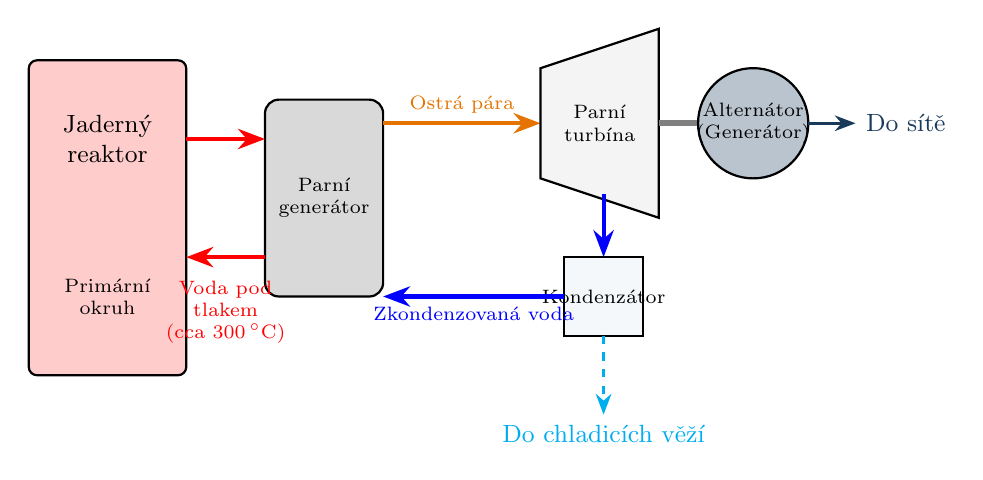
\begin{tikzpicture}[>=Stealth, font=\small, thick]
  % Primární okruh (červený)
  \draw[fill=red!20, rounded corners=3pt] (0,0) rectangle (2,4);
  \node[align=center] at (1,3) {Jaderný\\reaktor};
  \node[font=\scriptsize, align=center] at (1,1) {Primární\\okruh};

  % Parní generátor
  \draw[fill=gray!30, rounded corners=5pt] (3,1) rectangle (4.5,3.5);
  \node[align=center, font=\scriptsize] at (3.75,2.25) {Parní\\generátor};

  % Propojení primáru
  \draw[->, red, line width=1.5pt] (2,3) -- (3,3);
  \draw[<-, red, line width=1.5pt] (2,1.5) -- (3,1.5);
  \node[font=\scriptsize, red, align=center] at (2.5,0.8) {Voda pod\\tlakem\\(cca 300\,$^\circ$C)};

  % Sekundární okruh (modrý) - pára
  \draw[->, orange!90!black, line width=1.5pt] (4.5,3.2) -- (6.5,3.2);
  \node[above, font=\scriptsize, orange!90!black] at (5.5,3.2) {Ostrá pára};

  % Turbína
  \draw[fill=lightgray] (6.5,2.5) -- (8,2) -- (8,4.4) -- (6.5,3.9) -- cycle;
  \node[align=center, font=\scriptsize] at (7.25,3.2) {Parní\\turbína};

  % Hřídel a Generátor
  \draw[line width=2pt, gray] (8,3.2) -- (8.5,3.2);
  \draw[fill=accent!30, circle] (9.2,3.2) circle (0.7);
  \node[align=center, font=\scriptsize] at (9.2,3.2) {Alternátor\\(Generátor)};
  \draw[->, accent, line width=1pt] (9.9,3.2) -- (10.5,3.2) node[right] {Do sítě};

  % Kondenzátor
  \draw[fill=lightblue!50] (6.8,0.5) rectangle (7.8,1.5);
  \node[align=center, font=\scriptsize] at (7.3,1) {Kondenzátor};

  \draw[->, blue, line width=1.5pt] (7.3,2.3) -- (7.3,1.5); % Z turbíny
  \draw[->, blue, line width=1.5pt] (6.8,1) -- (4.5,1); % Zpět do PG
  \node[below, font=\scriptsize, blue] at (5.65,1) {Zkondenzovaná voda};

  % Chladicí okruh (do věží)
  \draw[->, dashed, cyan, line width=1pt] (7.3,0.5) -- (7.3,-0.5) node[below] {Do chladicích věží};
\end{tikzpicture}
\end{center}

\textbf{Vlastnosti:} Obrovský výkon, levný provoz, nulové emise CO$_2$, ale drahá výstavba a problém s ukládáním vyhořelého paliva. Pracují výhradně v základním zatížení sítě (nelze je rychle zapínat a vypínat).

% ================================================================
\subsection*{4. Vodní elektrárny (VE)}

Využívají polohovou (potenciální) energii vodních toků. Typicky se staví přehradní hráz.
Vodní elektrárny umí \textbf{najet na plný výkon v řádech desítek sekund}, proto jsou klíčové pro vykrývání \textbf{špiček} a regulaci frekvence v síti.

\begin{vzorcebox}
\textbf{Výkon vodní elektrárny:}
\[
P = \eta \cdot \rho \cdot Q \cdot g \cdot h \jednotka{W}
\]
kde $\eta$ = účinnost soustrojí, $\rho$ = hustota vody ($1000\,\mathrm{kg/m^3}$), $Q$ = průtok vody [m$^3$/s], $g$ = gravitační zrychlení ($9{,}81\,\mathrm{m/s^2}$), $h$ = využitelný spád [m].
\end{vzorcebox}

\textbf{Typy vodních turbín:}
\begin{itemize}
  \item \textbf{Kaplanova:} Tvar lodního šroubu s natáčivými lopatkami. Pro \textbf{malé spády} (jezy, řeky) a velký průtok.
  \item \textbf{Francisova:} Voda vstupuje radiálně (z boku) a vystupuje axiálně (dolů). Pro \textbf{střední spády} (přehrady, např. Orlík).
  \item \textbf{Peltonova:} Lžícovitá kola. Proud vody z trysky naráží do lžic. Pro \textbf{obrovské spády} (horská jezera, stovky metrů) a malé průtoky.
\end{itemize}

\textbf{Přečerpávací vodní elektrárna (PVE):} (např. Dlouhé Stráně). Funguje jako obří "baterie". V noci (když je elektřiny přebytek a je levná) \textbf{čerpá} vodu ze spodní nádrže nahoru. Přes den (když je elektřiny nedostatek) se voda pustí dolů a turbína \textbf{vyrábí} špičkovou energii.

% ================================================================
\subsection*{5. Sluneční / Fotovoltaické elektrárny (FVE)}

Jediný běžný zdroj, který nemá točivý generátor.
\textbf{Princip fotovoltaického jevu:} Využívá polovodičů (křemík) s přechodem PN (\textit{blíže v Okruhu 12: Polovodiče}). Fotony slunečního záření naráží do krystalické mřížky a vyrážejí z ní elektrony, čímž vzniká stejnosměrné napětí (DC).

\begin{center}
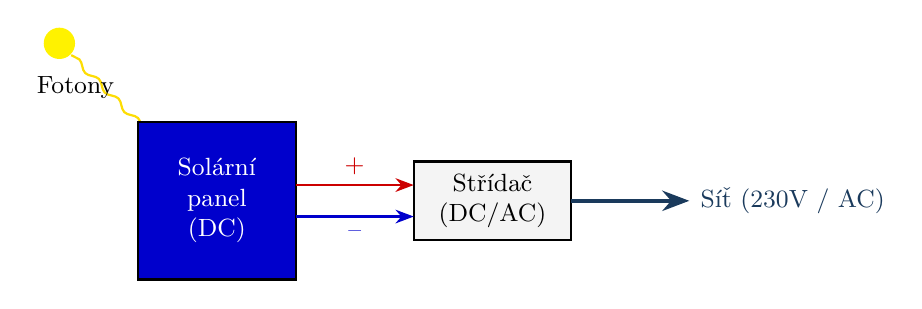
\begin{tikzpicture}[>=Stealth, font=\small, thick]
  % Slunce
  \node[circle, fill=yellow, inner sep=4pt] (sun) at (0,2) {};
  \draw[->, yellow!80!orange, decorate, decoration={snake, amplitude=1pt}] (sun) -- (1.5,0.5) node[midway, above left, text=black] {Fotony};

  % Panel
  \draw[fill=blue!80!black] (1, -1) rectangle (3, 1);
  \node[text=white, align=center] at (2,0) {Solární\\panel\\(DC)};

  % Střídač
  \draw[fill=lightgray] (4.5, -0.5) rectangle (6.5, 0.5);
  \node[align=center] at (5.5,0) {Střídač\\(DC/AC)};

  % Síť
  \draw[->, accent, line width=1.5pt] (6.5, 0) -- (8,0) node[right] {Síť (230V / AC)};

  % Dráty
  \draw[->, red!80!black] (3, 0.2) -- (4.5, 0.2) node[midway, above] {+};
  \draw[->, blue!80!black] (3, -0.2) -- (4.5, -0.2) node[midway, below] {--};
\end{tikzpicture}
\end{center}

\textbf{Střídač (Invertor):} Fotovoltaický panel dodává \textbf{stejnosměrný proud (DC)}, pro dodávku do sítě je nutné jej pomocí výkonové elektroniky převést na \textbf{střídavý proud (AC)} s frekvencí 50\,Hz zesynchronizovanou se sítí.

% ================================================================
\subsection*{6. Větrné elektrárny (VTE)}

Využívají kinetickou energii proudícího vzduchu. Vítr roztáčí rotor (většinou 3 listy), ten přes převodovku (nebo přímo) roztáčí generátor (často asynchronní nebo synchronní s permanentními magnety).
\textbf{Nevýhody FVE a VTE:} Dodávají energii \textbf{nepředvídatelně} (jen když fouká / svítí), což klade obrovské nároky na přenosovou soustavu a vyžaduje to záložní zdroje (např. plynové elektrárny), které pokryjí výpadky.

% ================================================================
\subsection*{7. Shrnutí – Porovnání zdrojů}

\begin{center}
\begin{tabularx}{0.97\linewidth}{@{} l X l l @{}}
\toprule
\textbf{Typ elektrárny} & \textbf{Režim v síti} & \textbf{Výhody} & \textbf{Nevýhody} \\
\midrule
\textbf{Jaderná} & Základní (24/7) & Levný provoz, bez CO$_2$, stabilita & Odpad, drahá a složitá stavba \\
\textbf{Tepelná (uhlí)} & Základní / Pološpičkový & Nezávislost na počasí, stabilita & Emise CO$_2$/SO$_2$, těžba \\
\textbf{Vodní} & Špičkový / Regulační & Rychlý start, ekologické, zdarma & Závislé na toku řek, povodně \\
\textbf{Větrná / Solární} & Nepředvídatelný & Zelená energie, nízké prov. náklady & Nestabilita výroby (počasí) \\
\bottomrule
\end{tabularx}
\end{center}

\end{vysvetlenibox}

\end{document}
